\documentclass{standalone}
\usepackage{tikz}
\usepackage{amsmath}
\usetikzlibrary{matrix}
\usetikzlibrary {shapes.geometric}
\usetikzlibrary {arrows.meta}
\begin{document}
    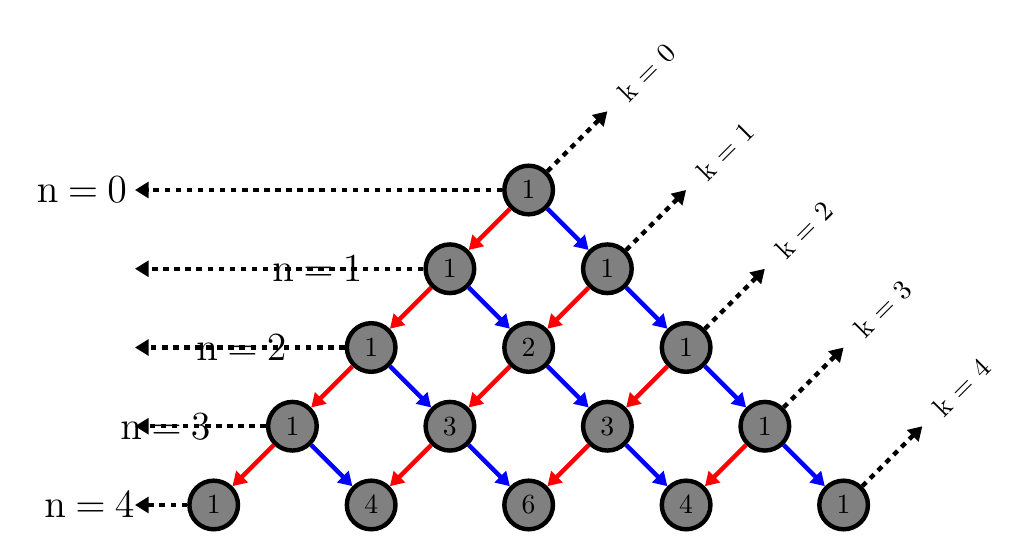
\begin{tikzpicture}[ultra thick]

        % \draw [help lines] (0,0) grid (13,6); 

        \path   (5,4) node (a) [circle,draw,fill = gray] {1}
                (4,3) node (b) [circle,draw,fill = gray] {1}
                (6,3) node (c) [circle,draw,fill = gray] {1}
                (3,2) node (d) [circle,draw,fill = gray] {1}
                (5,2) node (e) [circle,draw,fill = gray] {2}
                (7,2) node (f) [circle,draw,fill = gray] {1}
                (2,1) node (g) [circle,draw,fill = gray] {1}
                (4,1) node (h) [circle,draw,fill = gray] {3}
                (6,1) node (i) [circle,draw,fill = gray] {3}
                (8,1) node (j) [circle,draw,fill = gray] {1}
                (1,0) node (k) [circle,draw,fill = gray] {1}
                (3,0) node (l) [circle,draw,fill = gray] {4}
                (5,0) node (m) [circle,draw,fill = gray] {6}
                (7,0) node (n) [circle,draw,fill = gray] {4}
                (9,0) node (o) [circle,draw,fill = gray] {1};
            
        \draw[arrows = -{Triangle[open, angle=60:2mm,fill=red]},red]  (node cs: name =a ) -- (node cs:name =b);
        \draw[arrows = -{Triangle[open, angle=60:2mm,fill=blue]},blue] (node cs: name =a ) -- (node cs:name =c);
        \draw[arrows = -{Triangle[open, angle=60:2mm,fill=red]},red] (node cs: name =b ) -- (node cs:name =d);
        \draw[arrows = -{Triangle[open, angle=60:2mm,fill=blue]},blue] (node cs: name =b ) -- (node cs:name =e);
        \draw[arrows = -{Triangle[open, angle=60:2mm,fill=red]},red] (node cs: name =d ) -- (node cs:name =g);
        \draw[arrows = -{Triangle[open, angle=60:2mm,fill=red]},red] (node cs: name =c ) -- (node cs:name =e);
        \draw[arrows = -{Triangle[open, angle=60:2mm,fill=blue]},blue] (node cs: name =c ) -- (node cs:name =f);
        \draw[arrows = -{Triangle[open, angle=60:2mm,fill=red]},red] (node cs: name =g ) -- (node cs:name =k);
        \draw[arrows = -{Triangle[open, angle=60:2mm,fill=blue]},blue] (node cs: name =g ) -- (node cs:name =l);
        \draw[arrows = -{Triangle[open, angle=60:2mm,fill=blue]},blue] (node cs: name =d ) -- (node cs:name =h);
        \draw[arrows = -{Triangle[open, angle=60:2mm,fill=red]},red] (node cs: name =h ) -- (node cs:name =l);
        \draw[arrows = -{Triangle[open, angle=60:2mm,fill=red]},red] (node cs: name =e ) -- (node cs:name =h);
        \draw[arrows = -{Triangle[open, angle=60:2mm,fill=blue]},blue] (node cs: name =h ) -- (node cs:name =m);
        \draw[arrows = -{Triangle[open, angle=60:2mm,fill=blue]},blue] (node cs: name =e ) -- (node cs:name =i);
        \draw[arrows = -{Triangle[open, angle=60:2mm,fill=red]},red] (node cs: name =i ) -- (node cs:name =m);
        \draw[arrows = -{Triangle[open, angle=60:2mm,fill=blue]},blue] (node cs: name =i ) -- (node cs:name =n);
        \draw[arrows = -{Triangle[open, angle=60:2mm,fill=red]},red] (node cs: name =f ) -- (node cs:name =i);
        \draw[arrows = -{Triangle[open, angle=60:2mm,fill=blue]},blue] (node cs: name =f ) -- (node cs:name =j);
        \draw[arrows = -{Triangle[open, angle=60:2mm,fill=red]},red] (node cs: name =j ) -- (node cs:name =n);
        \draw[arrows = -{Triangle[open, angle=60:2mm,fill=blue]},blue] (node cs: name =j ) -- (node cs:name =o);
        
        
        \draw[arrows = -{Triangle[open, angle=60:2mm,fill=black]}] [dash pattern=on 2pt off 2pt](node cs: name =a ) -- (0,4);
        \draw[arrows = -{Triangle[open, angle=60:2mm,fill=black]}] [dash pattern=on 2pt off 2pt](node cs: name =b ) -- (0,3);
        \draw[arrows = -{Triangle[open, angle=60:2mm,fill=black]}] [dash pattern=on 2pt off 2pt](node cs: name =d ) -- (0,2);
        \draw[arrows = -{Triangle[open, angle=60:2mm,fill=black]}] [dash pattern=on 2pt off 2pt](node cs: name =g ) -- (0,1);
        \draw[arrows = -{Triangle[open, angle=60:2mm,fill=black]}] [dash pattern=on 2pt off 2pt](node cs: name =k ) -- (0,0);

        \node [left=4.1cm,text width=2cm] at (a)
        {
        \mbox{\Large n = 0}
        };

        \node [left=3.1,text width=2cm] at (b)
        {
        \mbox{\Large n = 1}
        };

        \node [left=2.1,text width=2cm] at (d)
        {
        \mbox{\Large n = 2}
        };

        \node [left=1.1,text width=2cm] at (g)
        {
        \mbox{\Large n = 3}
        };

        \node [left=0.1,text width=2cm] at (k)
        {
        \mbox{\Large n = 4}
        };

        \draw[arrows = -{Triangle[open, angle=60:2mm,fill=black]}] [dash pattern=on 2pt off 2pt](node cs: name =a ) -- (6,5);
        \draw[arrows = -{Triangle[open, angle=60:2mm,fill=black]}] [dash pattern=on 2pt off 2pt](node cs: name =c ) -- (7,4);
        \draw[arrows = -{Triangle[open, angle=60:2mm,fill=black]}] [dash pattern=on 2pt off 2pt](node cs: name =f ) -- (8,3);
        \draw[arrows = -{Triangle[open, angle=60:2mm,fill=black]}] [dash pattern=on 2pt off 2pt](node cs: name =j ) -- (9,2);
        \draw[arrows = -{Triangle[open, angle=60:2mm,fill=black]}] [dash pattern=on 2pt off 2pt](node cs: name =o ) -- (10,1);
        
        \node [right=1cm,text width=1cm , rotate = 45] at (5,5)
        {
        \mbox{ k = 0}
        };

        \node [right=1cm,text width=1cm , rotate = 45] at (6,4)
        {
        \mbox{ k = 1}
        };

        \node [right=1cm,text width=1cm , rotate = 45] at (7,3)
        {
        \mbox{ k = 2}
        };

        \node [right=1cm,text width=1cm , rotate = 45] at (8,2)
        {
        \mbox{ k = 3}
        };           

        \node [right=1cm,text width=1cm , rotate = 45] at (9,1)
        {
        \mbox{ k = 4}
        };


    \end{tikzpicture}
\end{document}